\documentclass[tikz,border=6pt]{standalone}
\usepackage[T1]{fontenc}
\usepackage{lmodern}
\usepackage{amsmath}
\usepackage{amssymb}
\usepackage{bm}
\usepackage{xcolor}
\usepackage{tikz}
\usetikzlibrary{arrows.meta,positioning,fit,calc,backgrounds,shapes.multipart,shapes.geometric}

\colorlet{mandalaBlue}{blue!55!black}
\colorlet{mandalaTeal}{teal!55!black}
\colorlet{mandalaGreen}{green!45!black}
\colorlet{mandalaGold}{orange!70!black}
\colorlet{mandalaRed}{red!55!black}
\colorlet{mandalaViolet}{violet!55!black}
\colorlet{mandalaGray}{black!55}
\colorlet{mandalaLight}{black!3}

\tikzset{
  >=Latex,
  font=\sffamily,
  % Color semantics used consistently across all diagrams:
  % mandalaBlue   -> external inputs / sources / configuration
  % mandalaTeal   -> internal data containers / encoded features
  % mandalaGreen  -> geometric or physics-aware transformations
  % mandalaGold   -> model computation or linear-algebra solve stages
  % mandalaViolet -> predicted operator-valued objects and heads
  % mandalaRed    -> optimization / objectives / losses
  titlebox/.style={
    rounded corners=2.5pt,
    fill=mandalaBlue!8,
    draw=mandalaBlue,
    line width=0.8pt,
    inner sep=6pt,
    minimum height=10mm,
    align=center,
    font=\sffamily\bfseries\large
  },
  panel/.style={
    rounded corners=3pt,
    fill=white,
    draw=black!45,
    line width=0.8pt,
    inner sep=5pt
  },
  stage/.style={
    rounded corners=3pt,
    fill=#1!10,
    draw=#1!85!black,
    line width=0.9pt,
    minimum width=32mm,
    minimum height=11mm,
    align=center,
    font=\sffamily\small
  },
  stage/.default=mandalaBlue,
  smallstage/.style={
    rounded corners=2.5pt,
    fill=#1!9,
    draw=#1!80!black,
    line width=0.75pt,
    minimum width=27mm,
    minimum height=8.5mm,
    align=center,
    font=\sffamily\scriptsize
  },
  smallstage/.default=mandalaBlue,
  sidepanel/.style={
    rounded corners=3pt,
    fill=#1!8,
    draw=#1!75!black,
    line width=0.8pt,
    inner sep=5pt,
    align=left,
    font=\sffamily\scriptsize,
    text width=43mm
  },
  sidepanel/.default=mandalaTeal,
  annot/.style={
    font=\sffamily\scriptsize,
    text=mandalaGray,
    align=left
  },
  arrow/.style={
    -{Latex[length=2.6mm,width=1.8mm]},
    line width=0.95pt,
    draw=black!70
  },
  dashedarrow/.style={
    -{Latex[length=2.4mm,width=1.7mm]},
    line width=0.85pt,
    draw=black!65,
    dashed
  },
  softfit/.style={
    rounded corners=4pt,
    draw=black!35,
    fill=black!1,
    line width=0.7pt,
    inner sep=6pt
  },
  lab/.style={
    font=\sffamily\scriptsize\bfseries,
    text=black!75
  },
  tinycode/.style={
    font=\ttfamily\tiny,
    text=black!70,
    align=center
  }
}

\begin{document}
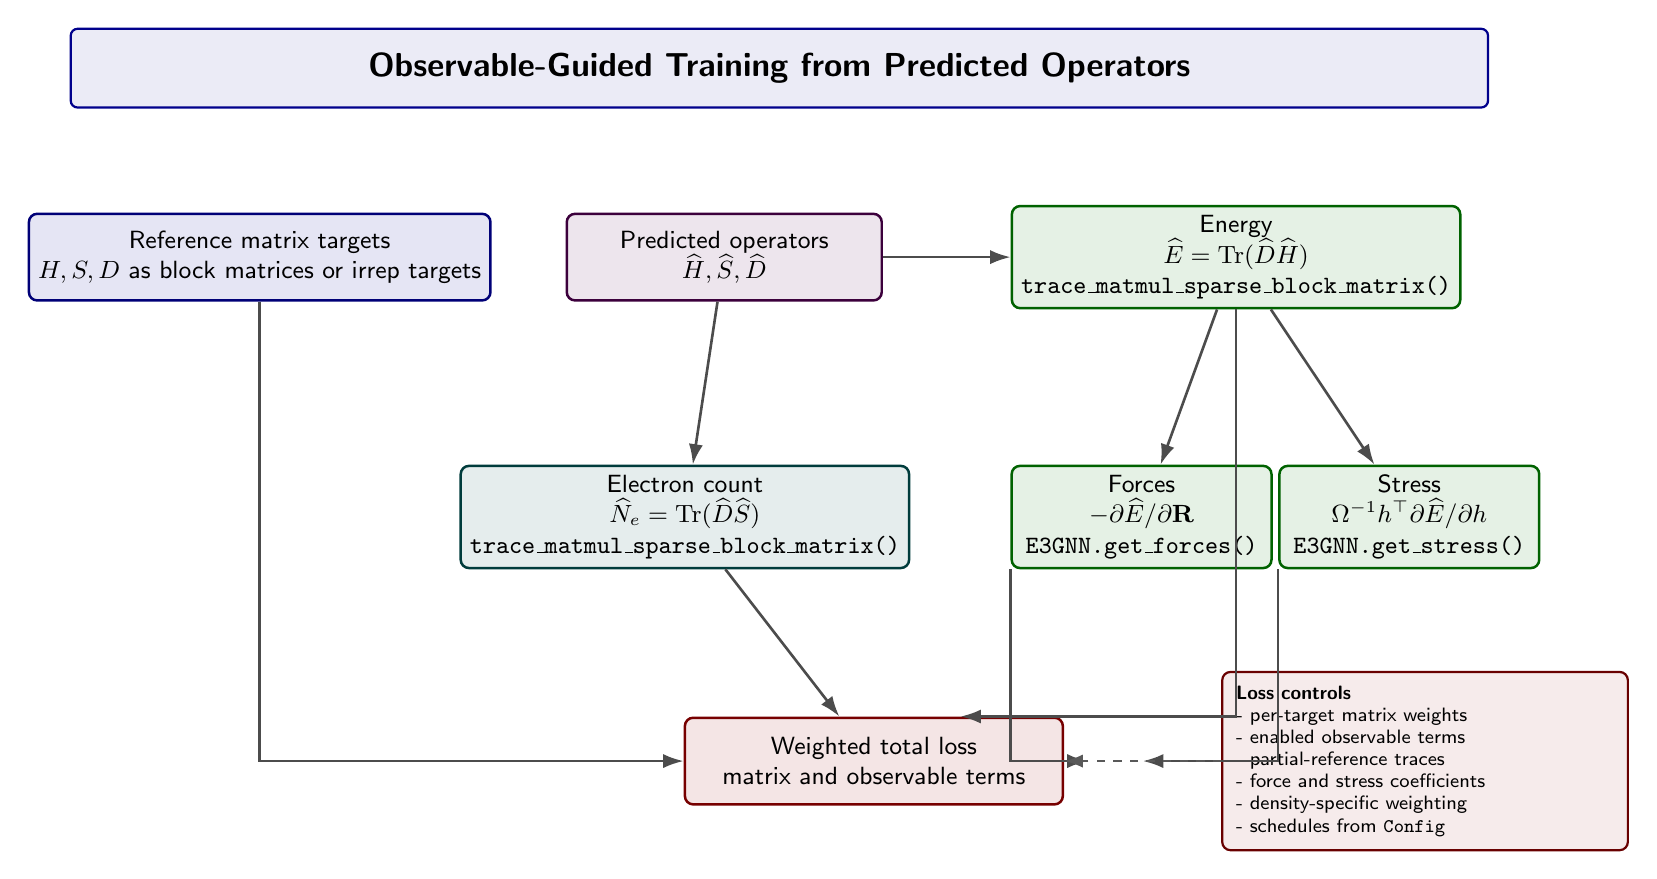
\begin{tikzpicture}[x=1cm,y=1cm]

\node[titlebox, minimum width=18.0cm] (title) at (0,0) {Observable-Guided Training from Predicted Operators};

\node[stage=mandalaBlue, minimum width=4.0cm] (mats) at (-6.6,-2.4)
{Reference matrix targets\\
$H,S,D$ as block matrices or irrep targets};
\node[stage=mandalaViolet, minimum width=4.0cm] (ops) at (-0.7,-2.4)
{Predicted operators\\
$\widehat{H},\widehat{S},\widehat{D}$};

\node[stage=mandalaGreen, minimum width=3.8cm] (energy) at (5.8,-2.4)
{Energy\\
$\widehat{E}=\mathrm{Tr}(\widehat{D}\widehat{H})$\\
\texttt{trace\_matmul\_sparse\_block\_matrix()}};
\node[stage=mandalaGreen, minimum width=3.3cm] (forces) at (4.6,-5.7)
{Forces\\
$-\partial \widehat{E}/\partial \mathbf R$\\
\texttt{E3GNN.get\_forces()}};
\node[stage=mandalaGreen, minimum width=3.3cm] (stress) at (8.0,-5.7)
{Stress\\
$\Omega^{-1} h^\top \partial \widehat{E}/\partial h$\\
\texttt{E3GNN.get\_stress()}};

\node[stage=mandalaTeal, minimum width=4.1cm] (nelec) at (-1.2,-5.7)
{Electron count\\
$\widehat{N}_e=\mathrm{Tr}(\widehat{D}\widehat{S})$\\
\texttt{trace\_matmul\_sparse\_block\_matrix()}};

\node[stage=mandalaRed, minimum width=4.8cm] (loss) at (1.2,-8.8)
{Weighted total loss\\
matrix and observable terms};

\node[sidepanel=mandalaRed, text width=4.8cm] (controls) at (8.2,-8.8)
{\textbf{Loss controls}\\
- per-target matrix weights\\
- enabled observable terms\\
- partial-reference traces\\
- force and stress coefficients\\
- density-specific weighting\\
- schedules from \texttt{Config}};

\draw[arrow] (mats.south) |- (loss.west);
\draw[arrow] (ops) -- (energy);
\draw[arrow] (ops) -- (nelec);
\draw[arrow] (energy) -- (forces);
\draw[arrow] (energy) -- (stress);
\draw[arrow] (energy.south) |- ([xshift=1.1cm]loss.north);
\draw[arrow] (nelec) -- (loss);
\draw[arrow] (forces.south west) |- ([xshift=0.3cm]loss.east);
\draw[arrow] (stress.south west) |- ([xshift=1.0cm]loss.east);
\draw[dashedarrow] (controls.west) -- (loss.east);

\end{tikzpicture}
\end{document}
